\chapter{Implementation Scenario}
 \begin{figure}[!htbp]
	\centering
	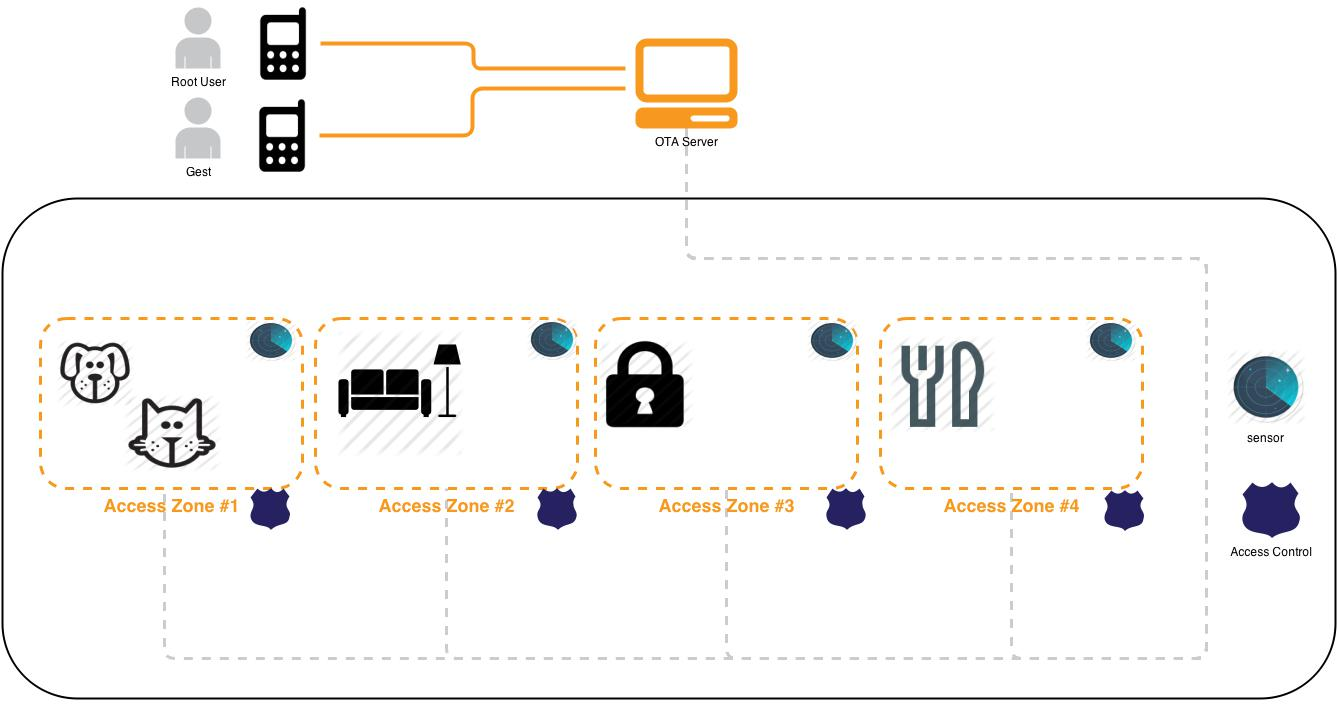
\includegraphics[width=1\textwidth]{homeoverview.jpg}
		\caption{Smart Home}
	\label{fig:SmartHome}
\end{figure}

\section{Overview}
Figure~\ref{fig:SmartHome} describes the basic structure and functionalities provided by implementation scenario, Smart Home. In the above-pictured housing scenario, following devices are introduced.
\begin{itemize}
\item Housing devices. Such as temperature sensors, coffee machine and digital door lock. They provide house holder a comfortable living condition by offering services such as:
\begin{itemize}
\item General device state query functionality.
\item Door lock access control management.
\item Home temperature and luminance management and coordination.
\item Notification and alert.
\end{itemize}
\item Smart Phone. The house holder with the help of smart phone is able to manage housing devices.
\item Remote Administrator server, whose duties are authenticate communication partners, public key management and secure messing.
\end{itemize}

\section {Component Structure}
 \begin{figure}[!htb]
	\centering
	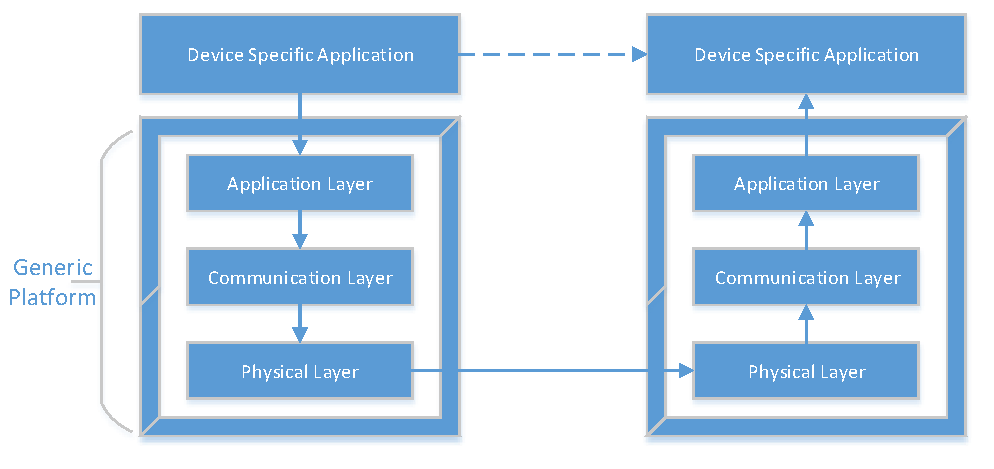
\includegraphics[width=1.1\textwidth]{component}
		\caption{Smart Home System Component Structure}
	\label{fig:SmartHomeComponent}
\end{figure}
With inspiration offered by application described  in section~\ref{secAgent}, in order to provide a generic application platform for vendor specific devices, my demonstration Smart Home system consists of components, \footnote{All housing devices that build the system and  smart phone are generically referred as system components.} whose basic structure is illustrated in figure~\ref{fig:SmartHomeComponent}.  As can be seen, components are composed of three layers. From bottom to top, they are:

\begin{itemize}
\item Physical layer. In this layer electronic devices and facilities are deployed. Alternatively lower level component could be also in this layer of higher level component.
\item Communication layer. Smart card and corresponding remote file/application management protocols together form this layer. The main responsibility of communication layer is to create a secure communication environment for application layer.
\item Application layer. OPC UA client application (installed on smart phone) and OPC UA server application (installed on other homing devices) are placed in this layer and provide a common interface for higher layer device specific application. 
\end{itemize}

Moreover this component platform also emphasizes the importance of secure messaging, peer authentication as well as authorization and provides corresponding secure mechanisms, which will be discussed in upcoming paragraphs.

 \begin{figure}[!htb]
	\centering
	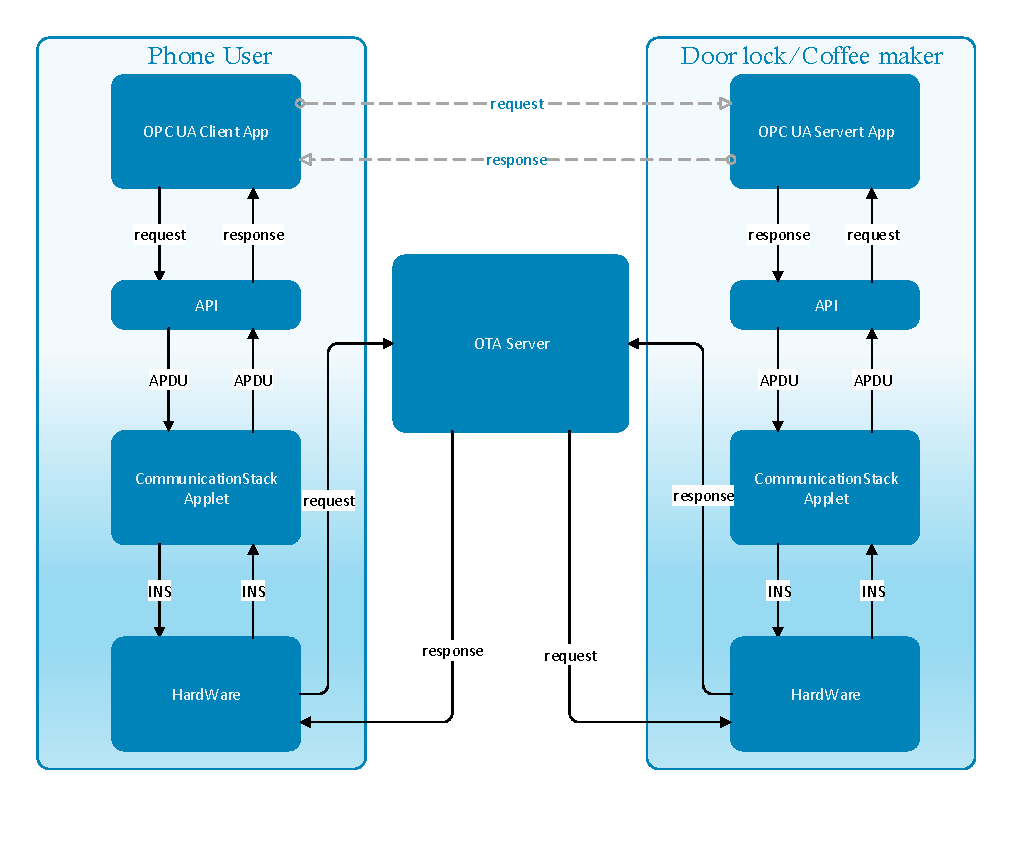
\includegraphics[width=1.1\textwidth]{csoverview}
		\caption{OPC UA Client Server Structure Example}
	\label{fig:softwareStructure}
\end{figure}

\section{Communication Flow}
Figure~\ref{fig:softwareStructure} pictures the communication flow between two system components. OPC UA Client and Server application communicate with each other with the help of an OTA server. And the communication stack is in charge of creation and managing secure communications between OTA server and secure devices. Moreover OPC UA client application is able to communicate with OPC UA server application using Short Message Service(SMS) or TCP/IP based web service. One demonstration case is given as below:

When the householder wants to make some coffee, he will send the \emph{makeCoffee} command to coffee maker with his cell phone in following steps as pictured in figure~\ref{fig:softwareStructure}. 
\begin{enumerate}
\item OPC UA Client application installed on cell phone initially generates the \emph{makeCoffee} request and forwards it to the internal API, such as openmobile API.
\item The internal API translates the request into remote APDU object, and the \emph{CommunicationStack} applet will try to connect with remote OTA server and forward this APDU commond to the OTA server.
\item OTA server will firstly in this step check the identification of the message sender.
\item After a successful identification, OTA server is able to confirm the cardholder's identify and to transmit his request to targeted message receiver.
\item  At last the \emph{makeCoffee} command will be received and performed by OPC UA server application installed on coffee maker. Alternatively it also generates a response message and notifies the phone user that his job is successful  finished. 
\end{enumerate}
The two core system parts involved in above described scenario are \emph{CommunicationStack applet} and \emph{OPC UA client/server application code} 

\subsection{CommunicationStack Applet}
Communication stack is integrated in UICC smart card, whose responsibility is realizing secure channel as well as session management, transporting data to receiver using TCP/IP connections or SMS. To be more specifically, the Communication stack's responsibilities are:
\begin{itemize}
  \item initiate Http session based on TLS(proactive)
  \item trigger Http session based on trigger SMS send by OTA server(passive)
  \item rebuild broken communication channel
  \item message encryption as well as decryption
  \item message transmit
\end{itemize}

Moreover thanks to self-containment structure, smart card itself does not dependent on other external resources, which could be extreme vulnerable to potential secure attack, and therefore provides a better hardware security and OS security. 

\subsection{OPC UA appliation Functionalities}\label{secFunction}
In conclusion, OPC UA server on secure housing device provides following services:
 \begin{itemize}
  \item processing client subscription/publishing environment data.
  \item secure message exchange with client.
  \item authority management.
  \item historical data record.
  \item execution client's command.
  \item Managing corresponding homing device.
\end{itemize}
Basic OPC UA client functions as following are provided by smart phone:
 \begin{itemize}
  \item submitting subscription/receiving published data.
  \item secure message exchange with server.
  \item sending command/configuration data.
  \item querying system historical data.
  \item providing user friendly interface.
\end{itemize}


 \begin{figure}[!htbp]
	\centering
	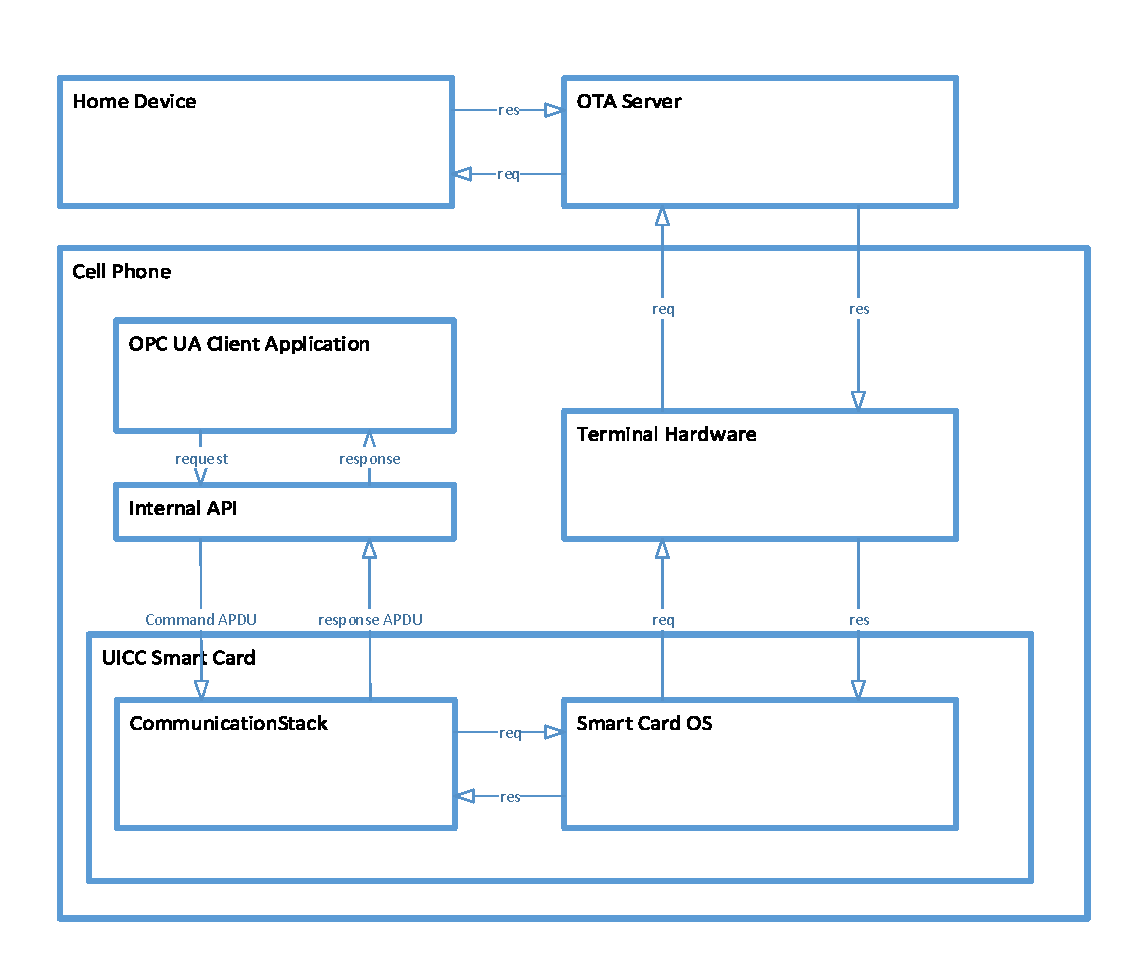
\includegraphics[width=0.78\textwidth]{clientStructure}
		\caption{Client Structure}
	\label{fig:clientStructure}
\end{figure}

\subsection{Cell Phone Side Software Structure}
As described in figure~\ref{fig:clientStructure}, the cell phone introduced in my application scenario consists of OPC UA client application code that realizes client application level functions, internal API, communication stack applet, smart card and phone hardware.

\begin{figure}[!htbp]
	\centering
	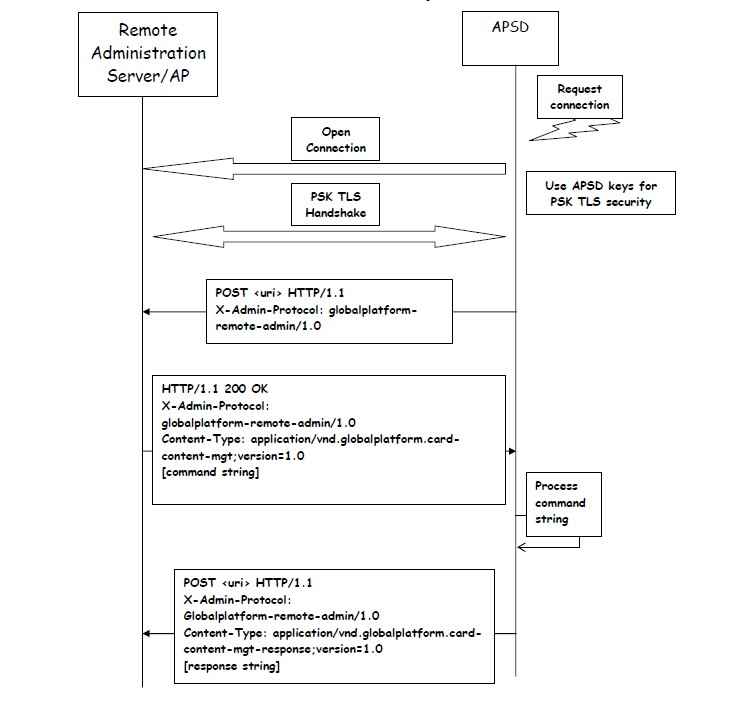
\includegraphics[width=1.2\textwidth]{apsd.jpg}
		\caption{Communication Flow between an AP and corresponding APSD\cite{ramGP}}
	\label{fig:apsd}
\end{figure}
The remote communication flow applied in my application scenario is compliant with the one provided by GlobalPlatform as shown in figure~\ref{fig:apsd}, who defines mechanisms for secure information exchange between a remote entity and a terminal, which is also known as Remote Application Management(RAM) over Http protocol and PSK TLS security. 

Application Security Domain(APSD) issued by GloablPlatform represents the terminal device in the realm of RAM and the aforementioned remote entity  is also referred as Remote Administration Server. 

With these two concepts, smart card holding the appropriate Security Domain can act as Http client and is capable of packing APDU formate information into Http POST message and transmitting Http message to OTA server, which will then forward this Http message to target receiver.\cite{ramGP}
 
Figure~\ref{fig:apsd} illustrates a typical RAM communication flow between administration server and corresponding security domain (Application Security Domain) on smart card. As can be seen, the request for open communication channel is usually initialized by security domain, which represents the phone user. After a successful secure handshake, the remote administration server and security domain are able to based on Http connection exchange request and response strings, which encapsulate APDU instructions. GlobalPlatform has also provided  a lists of API used to initialize authentication process, to configure algorithm and keys used for message encryption and decryption, to perform secure messaging and etc.

\subsection{Housing Device Software Structure}

\begin{figure}[!htbp]
	\centering
	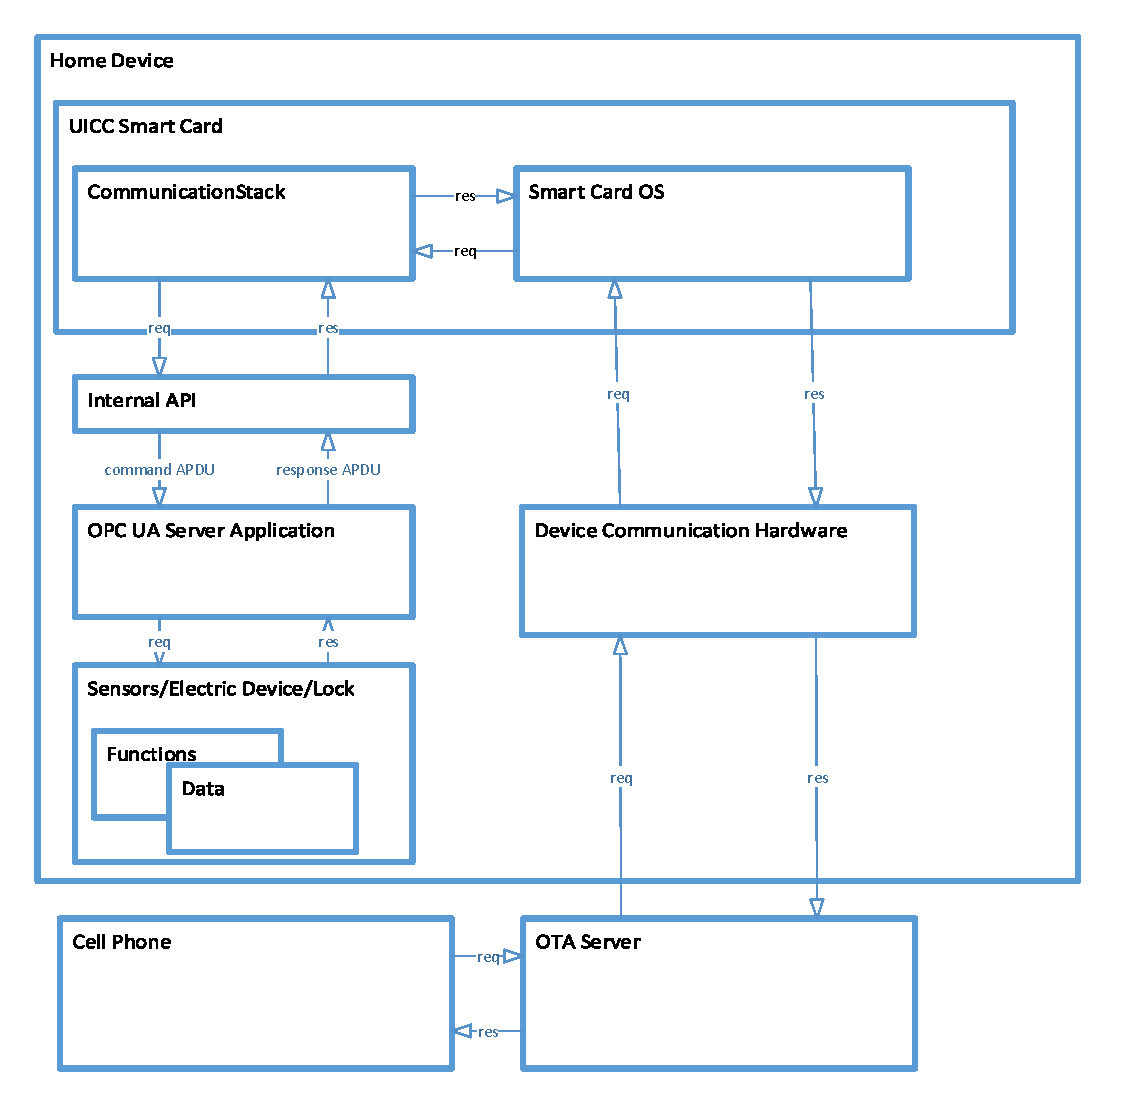
\includegraphics[width=0.85\textwidth]{serverStructure}
		\caption{Server Structure}
	\label{fig:serverStructure}
\end{figure}
Housing Device here refers to sensors, electric device as well digital locks that together build up the smart home. Each secure device provides services described in ~\ref{secFunction}. The device software structure is pictured as figure~\ref{fig:serverStructure} and it consists of OPC UA server application code, which offers basic functionalities like subscription and notification mentioned before, an internal API, an on smart card integrated communication stack and device specific functions as well as data.

\subsection{Implementation Tool Support}
\subsubsection{Java Card Application Design and Debug Tool}
Morpho presents JACADE with full name, Java Card Applet Develop Environment, which is more than just a IDE but a complex selection of various class APIs and software modules, that can be applied to design complete Java Card Applet as well as to debug Java source. 
\subsubsection{Java Card Applet Testing Environment}
When it comes to running test with Java Card Applet, tester has two options. Firstly, he can install the to be tested Applet on a smart card and then connection this chip card with test computer using \emph{Morpho Card Reader (MCR)}. Alternatively \emph{Java virtual card} which is integrated with test Applet also could be applied. 

In either way, as next step \emph{Universal Test Environment (UTE)} will be applied. \emph{UTE} provided by Morpho uses Java languages developed test cases
 and test scenarios\footnote{Test scenario is a collection of relative test cases.} to simulate desired use cases and observe corresponding smart card reactions. With the observed test result, tester will be able to analyze Applet's performance and debug corresponding application code. For instance \emph{UTE} can integrate software models used to simulate security domain offered by \emph{Globalplatform} and perform the sophisticate user authentication simulation process.
\subsubsection{Android Application Design Tool}
Eclipse IDE for Java Developer of version 3.7.1, together with Android SDK \emph{seek-for-android} and ADT plug-in,are applied as Android Application development environment. Moreover Android of version 2.3.5 is simulated and chosen as demonstration platform.
\subsubsection{Smart Home Simulation Environment}
In order to simulate data manged by home electronic device, \emph{MySQL} database is introduced. And together with \emph{PHP of version 5.5.12}, \emph{Apache of version 2.4.9}, the web server for Smart Home is created. Android Application from previous subsection will then communication with this web server for the purpose of scenario demonstration.